% !TEX root = ../main.tex
\chapter{Spannungsdoppelbrechung}

\begin{figure}[tb]
	\begin{subfigure}{.3\textwidth}
		\centering
		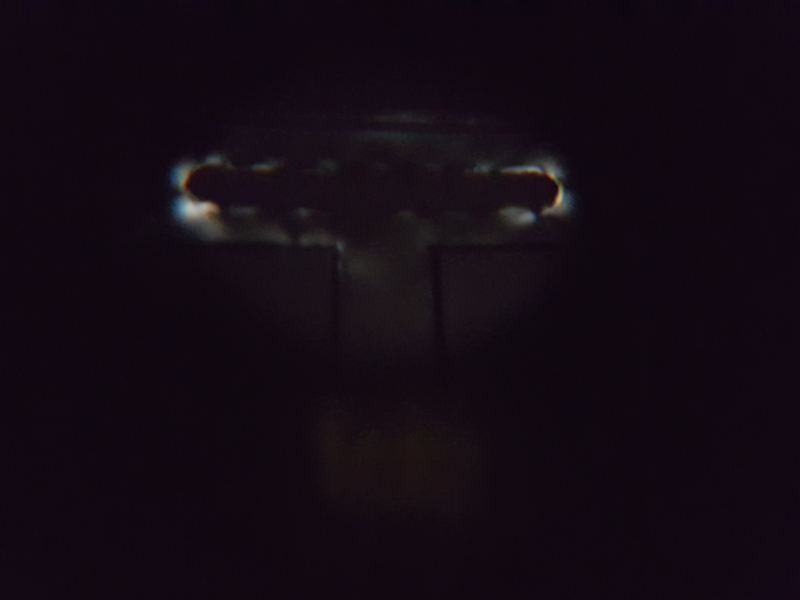
\includegraphics[height=.8\linewidth]{./img/tense1.jpg}
		\label{subfig:tensea}
	\end{subfigure}
	$\quad$
	\begin{subfigure}{.3\textwidth}
		\centering
		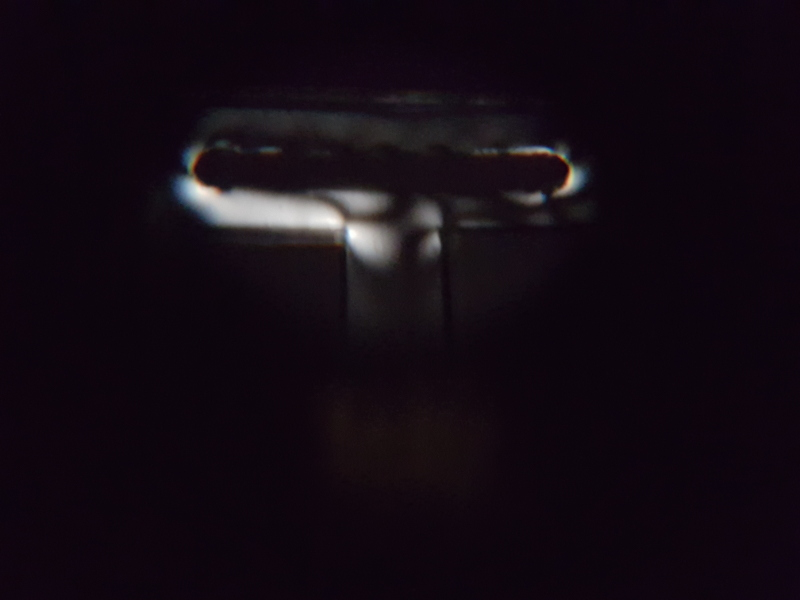
\includegraphics[height=.8\linewidth]{./img/tense3.jpg}
		\label{subfig:tenseb}
	\end{subfigure}
	$\quad$
	\begin{subfigure}{.3\textwidth}
		\centering
		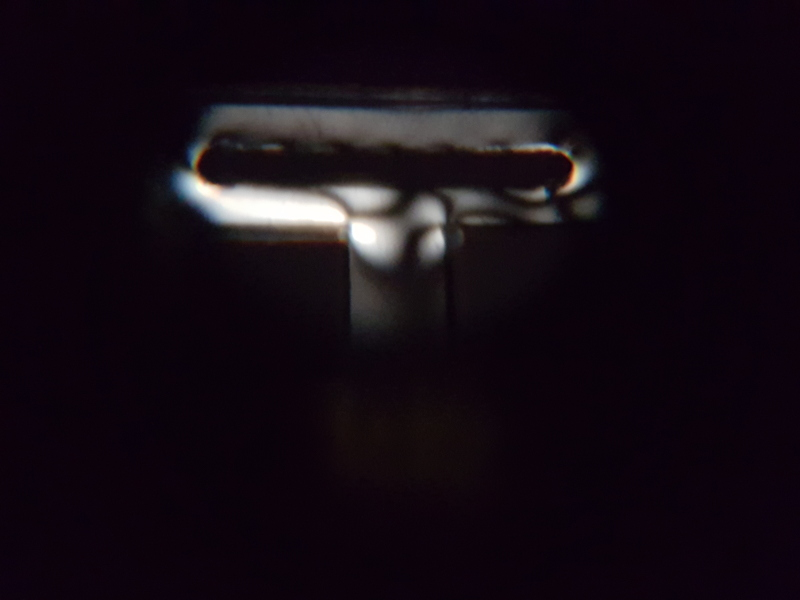
\includegraphics[height=.8\linewidth]{./img/tense2.jpg}
		\label{subfig:tensec}
	\end{subfigure}
	\caption[Spannungsdoppelbrechung am Plexiglasmodell]{Spannungsdoppelbrechung am Plexiglasmodell, v.l.n.r. stärker belastet}
	\label{fig:tense_without_crappy_joke}
\end{figure}

Bei vielen Materialen ändert sich bei mechanischer Beanspruchung die Brechzahl entlang der Deformationsache.
Dadurch tritt selbst an normalerweise isotropen Stoffen Doppelbrechung auf.
Die relative Stärke dieses Effektes ist abhängig von der Stärke der Verformung, daher können aus den Polarisationseigenschaften des Durchlichts Rückschlüsse über die lokale Belastung von Bauteilen gewonnen werden.

Am besten sichtbar ist dieser Effekt, wenn Polarisator und Analysator überkreuzt werden. Damit wird das gesamte Bild dunkel und nur Stellen stärkerer Belastung leuchten auf.

\autoref{fig:tense_without_crappy_joke} zeigt ein T-förmiges Plexiglasmodell mit einem schlitzförmigen Ausschnitt im Querbalken.